\documentclass{article}
\usepackage[margin=.5in]{geometry}
%\usepackage[utf8]{inputenc}
\usepackage{multicol}
\usepackage[boxruled,vlined]{algorithm2e}
\usepackage{verbatim}
\usepackage{hyperref}
\usepackage{graphicx}
\usepackage{float}
\usepackage{subcaption}

\graphicspath{{ ./ }}

\title{Defeated Zombies Through Deep Q-Learning in Minecraft}
\author{Hiroto Udagawa, Tarun Narasimhan, Shim-Young Lee}
\date{December 16, 2016}

\begin{document}
\maketitle

\begin{multicols}{2}

\section{Introduction}

In this project, we train an agent in the video game Minecraft with reinforcement learning to kill as many monsters as possible in a confined space. Our agent is only equipped with a sword to attack the monsters,  which can themselves attack and kill the agent.
The objective is to have the agent learn what policies to execute based on the visual information it receives about the surroundings from the raw pixels of the game play screen and the reward structure we have designed.
Using a convolutional neural network and Q-function reinforcement learning, the agent showed definite improvement in its ability to kill monsters.
This project displays the promise of combining deep learning with reinforcement learning to achieve non-trivial tasks.






\section{Related Work}

There have been several projects in this area which we drew upon for our project.
The major inspiration for our work was DeepMind's 2013 paper on deep reinforcement learning, in which the agent was trained with a single model architecture (Deep Q Learning) that uses convolutional neural network to perform a variant of Q-learning, and successfully played 7 different Atari 2600 games, in a few of which the agent outperformed human experts \cite{deepMind}.
Instead of solving the standard action-value function (Q function) with Bellman equation, deep convolutional neural network was used as a nonlinear function approximator, along with a biology inspired technique known as experience replay, which attempts to fix the divergence due to correlation between sequential inputs.
While a different network was trained for each game, the same architecture and hyperparameters were used across all of the games.
Furthermore, no prior (or game specific) knowledge was used, but only the raw pixel values were fed to the network as inputs.
DeepMind's major achievement was using extremely high-dimensional states (the visual input from the agent) and no information about the game rules to train an algorithm which could outperform skilled human players, and we aimed to replicate this in our project.

For the actual implementation of DeepMind's DQN in Python and TensorFlow, we relied heavily on Chen's work, which was also inspired by DeepMind's DQN and applied the same model architecture and algorithm to the game Flappy Bird \cite{flappyBird}.




\section{Minecraft and Project Malmo}

For the setting of our project, we chose Minecraft, a popular sandbox video game that was released in 2011. It allows players to control an agent, through which they can explore the map, build structures, craft tools, and destroy computer-generated monsters.
Project Malmo is an open source platform for Minecraft created by Microsoft that offers an interface for researchers to experiment with different approaches to artificial intelligence by controlling an agent through Python scripts.

Malmo is a useful environment for artificial intelligence research because it allows users to test endless situations within a relatively simple framework by  controlling agents' movements and environments via code.
By combining different states, actions, and spaces, researchers can create different environments and define various tasks for which the agent trains with reinforcement learning.

As a simulator, Malmo is more constrained than many other simulators which researchers have employed. Microsoft designed Malmo to be an interface with Minecraft, but not to provide the agent with any information about Minecraft.
Thus, the default in Malmo is for the player-controlled agent to not have any information about its environment or the rules of the game.
This feature makes Malmo very convenient for reinforcement learning as this replicates the exact kind of environment we want for reinforcement learning: in order to maximize difficulty, the agent should be trained only from its own visual input.
For example, the agent does not "know" that the \emph{attack} action kills zombies; it learns this through training.

[{\bf Hiro: do you want to discuss Minecraft/Malmo implementation issues here? Like the lag issue?}]




\section{Method}



\subsection{Scenario}

The agent begins in the middle of a completely flat room with a fixed number of randomly generated zombies. The room has a uniform color so that the algorithm will not have to account for differences in lighting and colors. The zombies automatically approach the agent and damage it if they get too close. The agent will be equipped with a sword to fend off the zombies. As the agent destroys zombies, new zombies continue to spawn (so that there is always a constant number of zombies), and the game continues to run until the character loses all of its health. At this time, the score will be calculated based on the total number of zombies that the character was able to kill and the scenario resets to the beginning.


\subsection{MDP Formulation}
 
We formalize the reinforcement learning task with Markov Decision Process. The agent interacts with an environment by making observations and actions, and receiving rewards. At each iteration, the agent selects an action from the action space, A = {1, . . . , K }. Agent's action in turn changes the state the agent is in and the agent receives rewards based on the new state it enters. The reward often depends not only on the new state it just entered, but the entire sequence of actions and observations it made until it entered state in which it received rewards. Thus, to make an appropriate action in the current state, the agent needs information from previous actions and observations as well as the current observation. We therefore consider sequences of actions and observations st = x1, a1, x2, ..., a(t-1), xt. All such sequences are finite, thus we now have finite Markov decision process (MDP), where we use the sequence st as a distinct state at each time-step t.

\subsubsection{Actions and States}

The actions for this problem are the discrete movements of the agent (the agent can move forward, back, turn left, turn right, or remain stationary) as well as the ability to attack with a sword. To simplify the action space, the attack command was turned on the entire time, and the agent only chooses how to move at each time-step. Minecraft allows the agent to move and turn with different speed, but we only use five possible actions with fixed moving and turning speed.

The observation at time-step t xt is an image of the player's vision represented by the pixels values. Project Malmo provides the functionality to retrieve the image from the screen. As stated earlier, the state at time-step t is a sequence of observations and actions made until and at time t. 

\begin{figure}[H]
\caption{Minecraft screenshot}
\centering
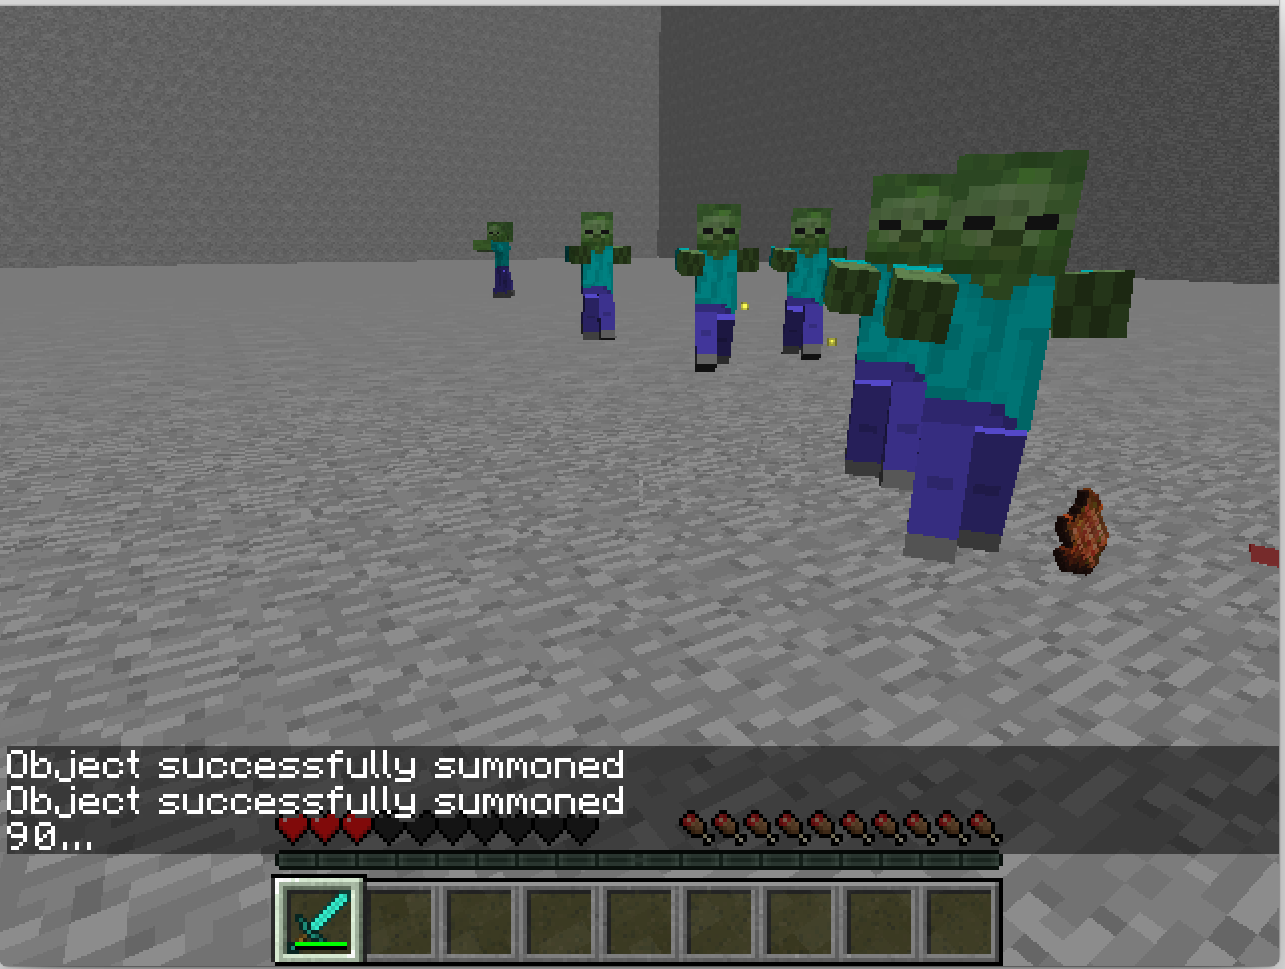
\includegraphics[scale=0.3]{./hiro_screenshot.png}
\end{figure}



\subsubsection{Reward}

We assign the algorithm a reward of +1 for a successful hit on a monster and a reward of +5 for a successful kill.
There is also a reward of 0.03 for every frame for which it stays alive and a penalty of -1 for every time the agent gets hit. These are designed to train the agent's behavior to incentivize staying alive; holding the kill count equal, we wanted the agent to have a higher reward for staying alive longer.


\subsection{Q-learning and Deep Q Network}

\subsubsection{Reinforcement Learning Background}

In reinforcement learning, the agent is to trained to maximize the aggregate future rewards. With the discount factor of \gamma, the future discounted return at time t is Rt = (HERE: sum of discounted returns), where T is the number of time-steps (or iterations) in that episode of the game. We define the optimal action-value function Q*(s, a) = max⇡ E [Rt|st = s, at = a, \pi], which is the maximum expected return achievable by following any strategy, after seeing some sequence s and then taking some action a, where \pi is a policy mapping sequences to actions (or distributions over actions).

In simpler settings, the optimal policy is obtained by solving the Bellman equation iteratively, using the equation Qi+1(s,a) = E [r +   maxa0 Qi (s0 , a0 )|s, a]. However, maintaining estimates of action-value function for all sequences(states) is impossible and yields no generalization for newly encountered states. Instead, we use convolutional neural network as a nonlinear function approximator to estimate the action-value function. We train the neural network approximator Q(s,a,\theta) by minimizing a loss functions L_i(theta) defined for each iteration i:

Li (✓i) = Es,a⇠⇢(·) h(yi   Q (s, a; ✓i))2i

where yi = Es0⇠E [r +   maxa0 Q(s0, a0; ✓i 1)|s, a] is the target for iteration i and p(s, a), the behaviour distribution, is a distribution over states s and actions a. Note that the target value used in iteration i is calculated with the previous iteration's network weights. For faster computation at each iteration, stochastic gradient descent is used; instead of calculating the expectation, we update the weights with a single sample from distribution. 

\subsubsection{Deep Q Network}

Since the observation the agent receives is an image (pixel values) of the gameplay screen, convolutional neural network is a reasonable choice of neural network. Although in the formulation of the MDP we stated that each state is an entire sequence of actions and observations, neural networks can only handle  

\subsubsection{experience replay}

\subsubsection{e-greedy policy}

the behaviour distribution is ofte e-greedy strategy that follows the greedy strategy with probability 1-e and selects a random action with probability e.


\subsection{Training}

\subsubsection{Preprocessing}

\subsubsection{Model Architecture}

\subsubsection{Algorithm}

must be able to learn from a scalar reward signal that is frequently sparse, noisy and delayed.

The delay between actions and resulting rewards, which can be thousands of timesteps long, seems particularly daunting when compared to the direct association between inputs and targets found in supervised learning. Another issue is that most deep learning algorithms assume the data samples to be independent, while in reinforcement learning one typically encounters sequences of highly correlated states.


We use Q-learning to have our agent learn a policy to best fight these monsters.
We utilize the work done by Google Deep Mind to use a convolutional neural network to approximate the Q-function iteration after iteration.
\paragraph{}


\begin{algorithm*}[H]
     \SetAlgoLined
     initialize Q function with random weights \;
     observe initial state $S$ \;
     \Repeat{terminated} {
        with probability $\epsilon$ generate random action \;
        otherwise select $a = \arg\max_{a'} Q(s,a')$ \;
        carry out action $a$ \;
        observe reward $r$ and new state $s'$ \;
        update $D$ with new data: $<s,a,r,s'>$ \;
        sample random transitions from $D$ \;
        update network \;
     }
     \caption{Adapted from Matiisen, 2015}
\end{algorithm*}

\begin{figure}[H]
\caption{Images of processed features}
\begin{subfigure}{.25\textwidth}
  \centering
  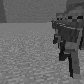
\includegraphics[scale=1.0]{./messigray1.png}
  \caption{1a}
  \label{fig:sfig1}
\end{subfigure}%
\begin{subfigure}{.25\textwidth}
  \centering
  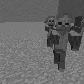
\includegraphics[scale=1.0]{./messigray2.png}
  \caption{1b}
  \label{fig:sfig2}
\end{subfigure}
\vskip\baselineskip
\begin{subfigure}{.25\textwidth}
  \centering
  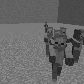
\includegraphics[scale=1.0]{./messigray3.png}
  \caption{1b}
  \label{fig:sfig3}
\end{subfigure}
\begin{subfigure}{.25\textwidth}
  \centering
  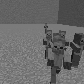
\includegraphics[scale=1.0]{./messigray4.png}
  \caption{1b}
  \label{fig:sfig4}
\end{subfigure}
\label{fig:fig}
\end{figure}



\section{Results and Analysis}

The agent kicks ass and takes names like Chuck Norris on cocaine.

\begin{description}
    \item[Table 1: Learning rate under varying Reward Structures]
    \item[Table 2: Learning rate under varying $\epsilon$]
    \item[Table 3: Learning rate under varying learning rates]
    \item[Table 4: Learning rate under varying difficulties]
\end{description}

We ran into the unexpected problem that...





\section{Conclusions and Future work}
We succesfully trained a Deep Q Network to move around a room and kill zombies by taking visual input from the agent.
Our results suggest that \emph{foo} and \emph{bar} methods worked best because [...]

Future work on this task might focus on expanding the agent's action space so that the agent can execute continuous movements rather than the discretized actions we have programmed.
Additionally, researchers could focus on improving DeepMind's convolutional neural network to further enhance the performance or learning curve of the algorithm.
This might involve different gradient algorithms or initial weights.

\end{multicols}





%%%%%%%%%%%%%%%%%%%%%%%%%%%%%%%%%%%%%%%%%%%%%%%%%%%%
%%%%%%%%%%%%%%%%%%% Bibliography %%%%%%%%%%%%%%%%%%%
%%%%%%%%%%%%%%%%%%%%%%%%%%%%%%%%%%%%%%%%%%%%%%%%%%%%
\pagebreak
\begin{thebibliography}{9}


\bibitem{deepMind}
Mnih, Volodymyr; Kavukcuoglu, Koray; Silver, David; Graves, Alex; Antonoglou, Ioannis; Wierstra, Daan; Riedmiller, Martin.
\emph{Playing Atari with Deep Reinforcement Learning},
December 2013.

\bibitem{nervanasys}
Matiisen, Tambet.
\emph{Demystifying Deep Reinforcement Learning}. December 2015.
\url{https://www.nervanasys.com/demystifying-deep-reinforcement-learning/}

\bibitem{flappyBird}
Chen, Kevin.
\emph{Deep Reinforcment Learning for Flappy Bird}


\end{thebibliography}


\end{document}
